%%%%%%%%%%%%%%%%%%%%%%%%%%%%%%
%%  Design pattern creazionali
%%%%%%%%%%%%%%%%%%%%%%%%%%%%%%

\begin{figure} \label{fig:injector}
	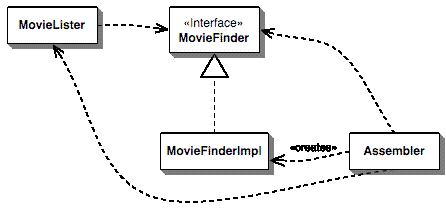
\includegraphics[scale=0.5]{img/injector}
	\caption{Dependency Injection.}
\end{figure}

\subsection{Dependency injection}

\subsubsection{Scopo} permette di disaccoppiare degli oggetti in modo da non dover modificare un oggetto se viene cambiato un altro su cui dipende, semplificando perciò lo sviluppo di un software di grandi dimensioni e allo stesso tempo migliorandone la testabilità.

\subsubsection{Motivazione} grazie a questo pattern è possibile separare la responsabilità di uso e creazione di un oggetto. Il componente dipendente dovrà solo sapere come usare un servizio richiesto,mentre il compito di creare ed iniettare quest'ultimo spetta ad un injector. Questo permette al componente dipendente di essere altamente configurabile in quanto è fisso solo il suo comportamento.

\subsubsection{Struttura} Sono coinvolti 3 componenti nella dependency injection:
\begin{itemize}
	\item gli oggetti servizi(ossia un qualsiasi oggetto che potrebbe essere usato);
	\item l'oggetto dipendente da questi servizi;
	\item un injector responsabile di creare ed iniettare i servizi.
\end{itemize}

\subsubsection{Applicabilità} è possibile applicare il pattern in tre modi differenti:
\begin{itemize}
	\item \textbf{setter injection:} la dipendenza viene iniettata tramite dei metodi setter del component dipendente;
	\item \textbf{costruction injection:} la dipendenza viene iniettata tramite un paramento del costruttore;
	\item \textbf{interface injection:} l'iniezione viene eseguita attraverso l'interfaccia che fornirà un setter a chiunque la implementa.
\end{itemize}
